\begin{figure*}[t]
\centering
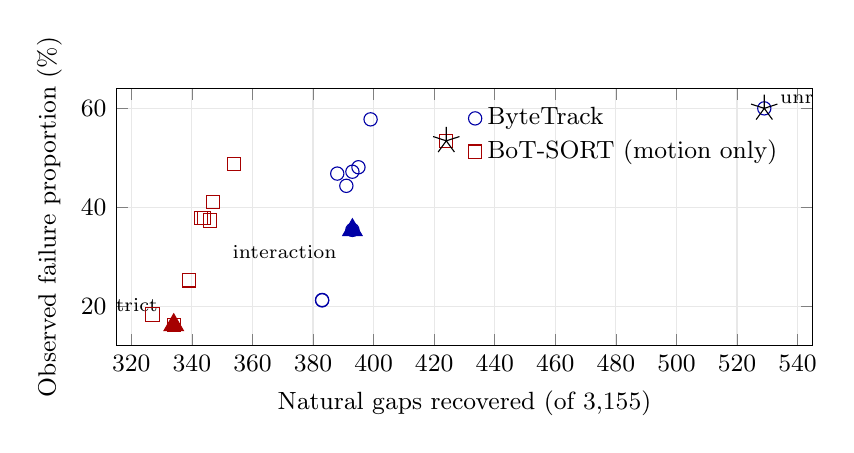
\begin{tikzpicture}
\begin{axis}[
    width=0.86\textwidth,
    height=0.40\textwidth,
    xlabel={Natural gaps recovered (of 3,155)},
    ylabel={Observed failure proportion (\%)},
    xmin=315, xmax=545,
    ymin=12, ymax=64,
    grid=major,
    grid style={gray!18},
    legend pos=north east,
    legend cell align=left,
    legend style={draw=none, fill=none, font=\small},
    tick label style={font=\small},
    label style={font=\small},
    mark size=2.4pt,
]
\addplot[only marks, mark=o, mark options={solid}, color=blue!65!black,
         forget plot] coordinates {
    (529,59.95) (399,57.73) (388,46.77) (391,44.30) (395,48.05)
    (393,35.39) (393,47.15) (383,21.15) (383,21.24)
};
\addlegendimage{only marks, mark=o, color=blue!65!black}
\addlegendentry{ByteTrack}
\addplot[only marks, mark=square, mark options={solid}, color=red!65!black,
         forget plot] coordinates {
    (424,53.39) (354,48.69) (343,37.76) (347,41.02) (339,25.19)
    (346,37.28) (344,37.78) (327,18.31) (334,16.19)
};
\addlegendimage{only marks, mark=square, color=red!65!black}
\addlegendentry{BoT-SORT (motion only)}
\addplot[only marks, mark=star, mark size=5pt, color=black] coordinates {(529,59.95)};
\addplot[only marks, mark=star, mark size=5pt, color=black] coordinates {(424,53.39)};
\addplot[only marks, mark=triangle*, mark size=4pt, color=blue!65!black] coordinates {(393,35.39)};
\addplot[only marks, mark=triangle*, mark size=4pt, color=red!65!black] coordinates {(334,16.19)};
\node[font=\scriptsize, anchor=south west] at (axis cs:531,59.0) {unrestricted};
\node[font=\scriptsize, anchor=north east] at (axis cs:391,34.2) {interaction};
\node[font=\scriptsize, anchor=south east] at (axis cs:332,16.9) {strict};
\end{axis}
\end{tikzpicture}
\caption{Every evaluated policy on the official PersonPath22 test subset,
plotted by the number of natural gaps it recovers and the observed
proportion of failed evaluated reactivations. Stars mark the unconstrained
trackers, triangles the relaxed interaction gate, and the lower-left
cluster the strict ceilings. Policies to the right of a given point recover
more gaps; policies below it fail less often. The frontier runs from the
strict ceilings at the lower left to the unconstrained tracker at the upper
right, so no single policy is best on both axes.}
\label{fig:tradeoff}
\end{figure*}
